\section{Stator Analysis: Origin of Cracking}
\label{Chap:stator_analysis}
The stator is exposed to two different thermal circumstances: operational and shut-down. This chapter will discuss the critical points of the stator for both conditions along with the origin of the cracking.

\subsection{Shut-down conditions}

The origin of cracking for shutdown conditions, meaning that the middle part of the stator is 150 [\textdegree C], is found using FEM-analysis. To find the origin of cracking, a thermo-elastic analysis is completed for the stator \cite{thermo-elasticity}. The maximum principal stress of the stator after this analysis can be seen in Figure \ref{stator1}. The location of the first cracking point is on the leading edge of the blade, where the blade attaches to the upper part of the stator. It is assumed that the point with the highest maximum principal stress is where the stator will crack first. For analyzing the stress in the stator and also in the improved design, the maximum principle stress will be used. This theory, also known as the Rankine criterion, predicts the failure of brittle materials, so this can be used to define when the stator starts to crack \cite{Solidmechanics}.

\begin{figure} [H]
 	\centering
 	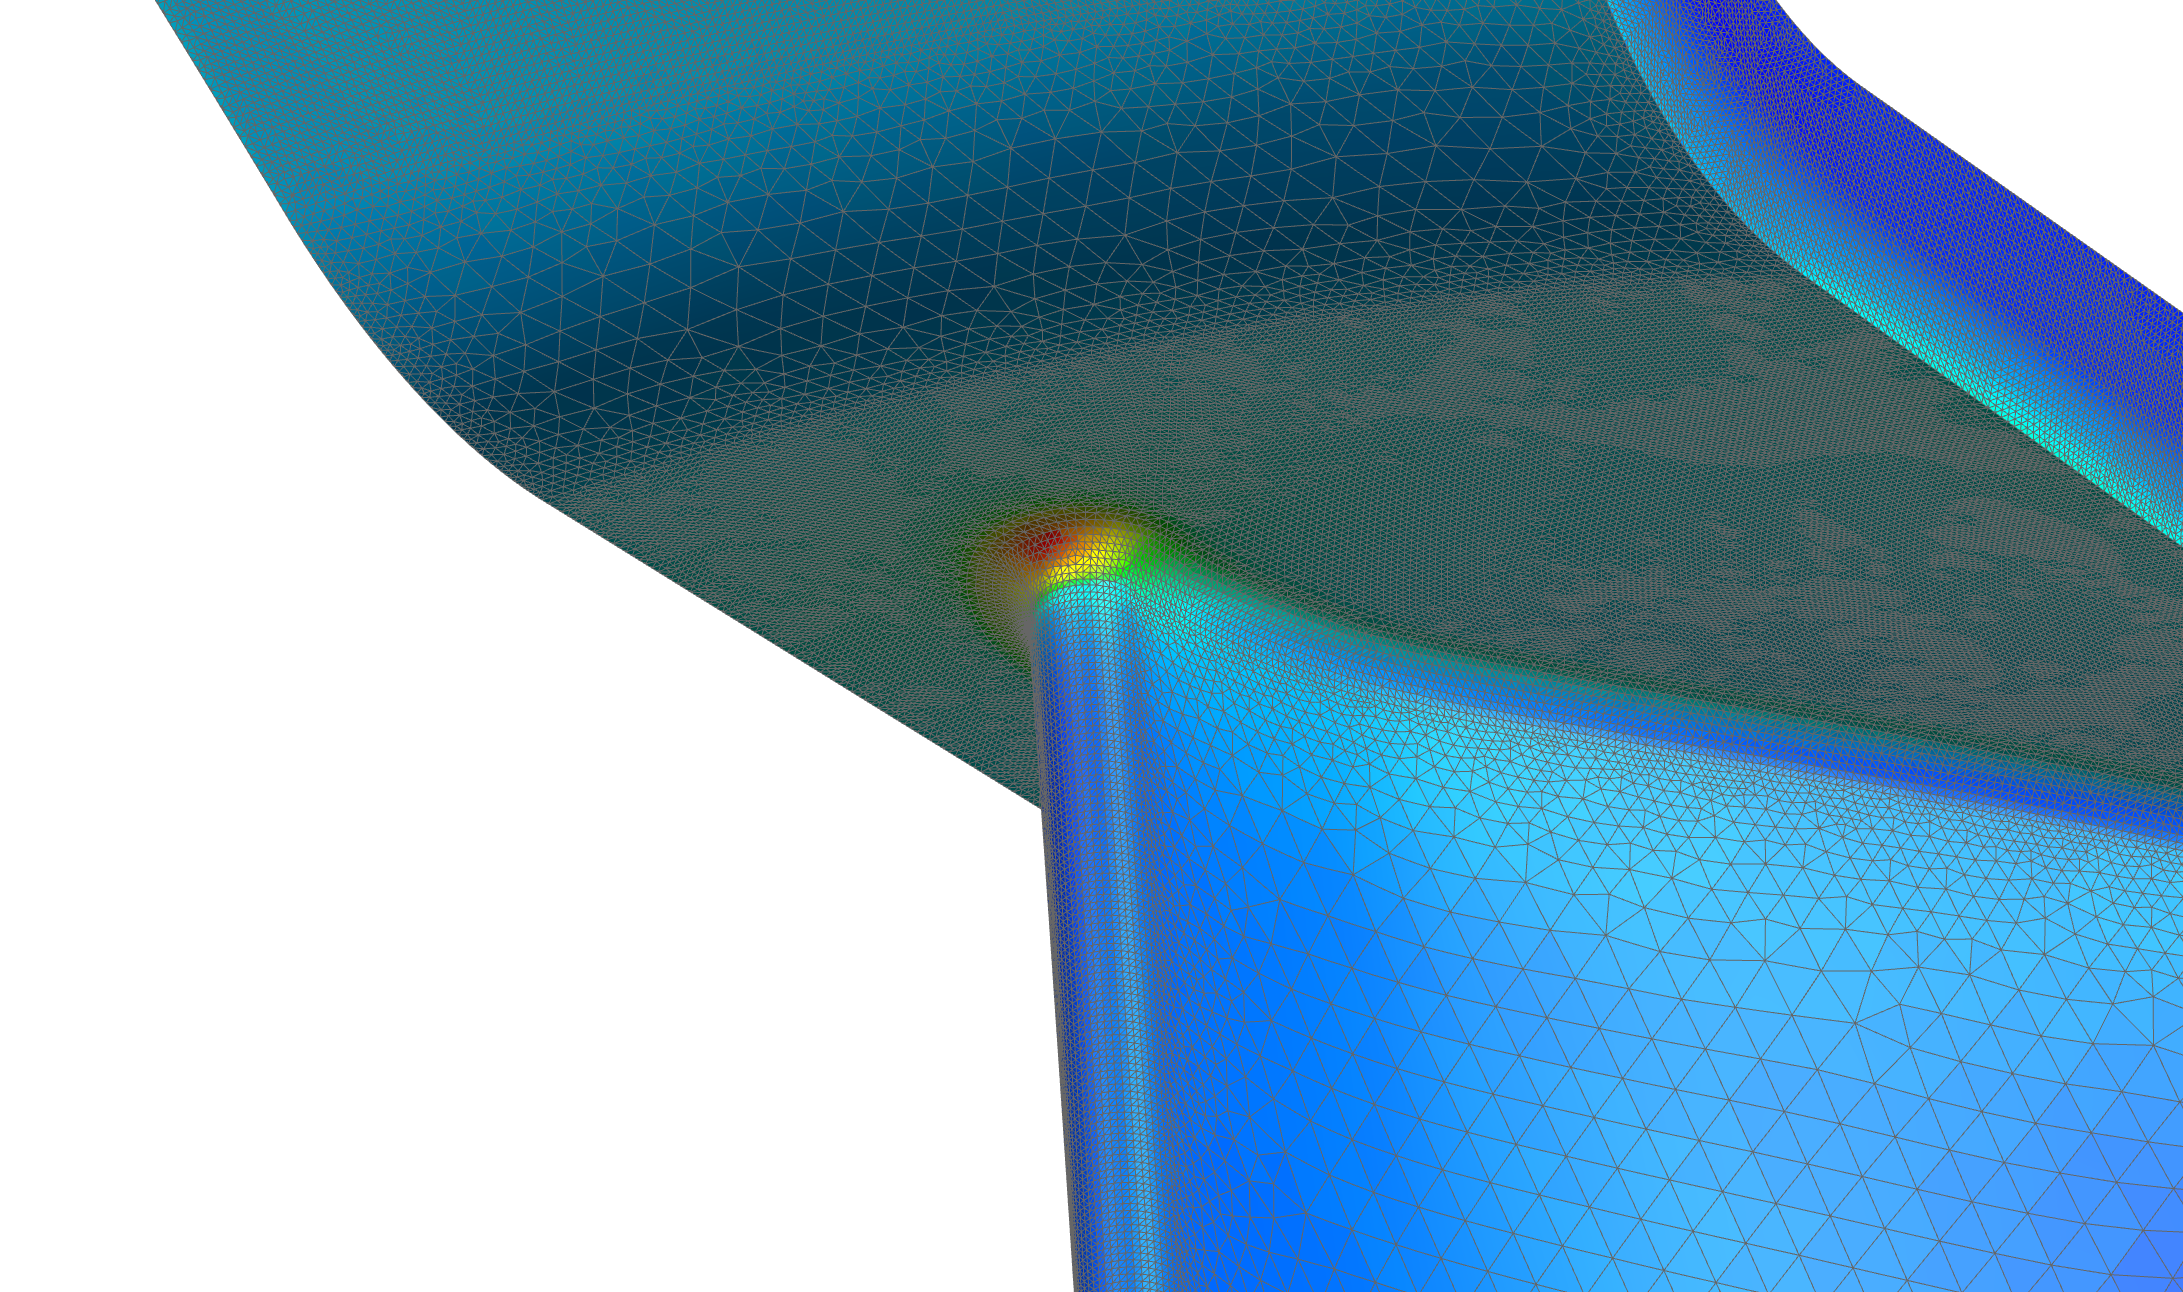
\includegraphics[width=0.8\linewidth]{Figures/stator_shutdown.png}
 	\caption{Maximum stress during shut-down condition}
    \label{stator1}
 \end{figure}

The reason that the stator will crack at this location first is related to the stress due to the temperature difference between the blade and the upper part of the stator. During shut-down conditions, there is a 500 [\textdegree C[] difference between these two. This will cause the upper part of the stator to expand more than the blade below. The upper part of the stator tries to expand in all directions, so it pulls on the upper part of the blade. The blade, especially at the leading edge, does not have a lot of material to prevent this expansion; this causes much tension at the top part of the blade. 

The highest stress found during the shut-down condition is near 2616 [MPa] when considering nodal stress, 2380 [MPa] when considering elemental stress. This value is valid due to the fact that it has a convergence percentage of 9 \%. This percentage is below the 10 \% convergence which is aimed for. See Appendix \ref{AppendixD} for  information about convergence.

\subsection{Operating conditions}
The origin of cracking for operating conditions, where the middle part of the stator is 750 [\textdegree C], is also determined using FEM-analysis. After completing a thermo-elastic analysis and checking for the highest principle stress, the cracking point is found to be at the edge between the bottom backside of the stator and the thin tail part of the stator, as can be seen in Figure \ref{stator2}. 

\begin{figure} [H]
 	\centering
 	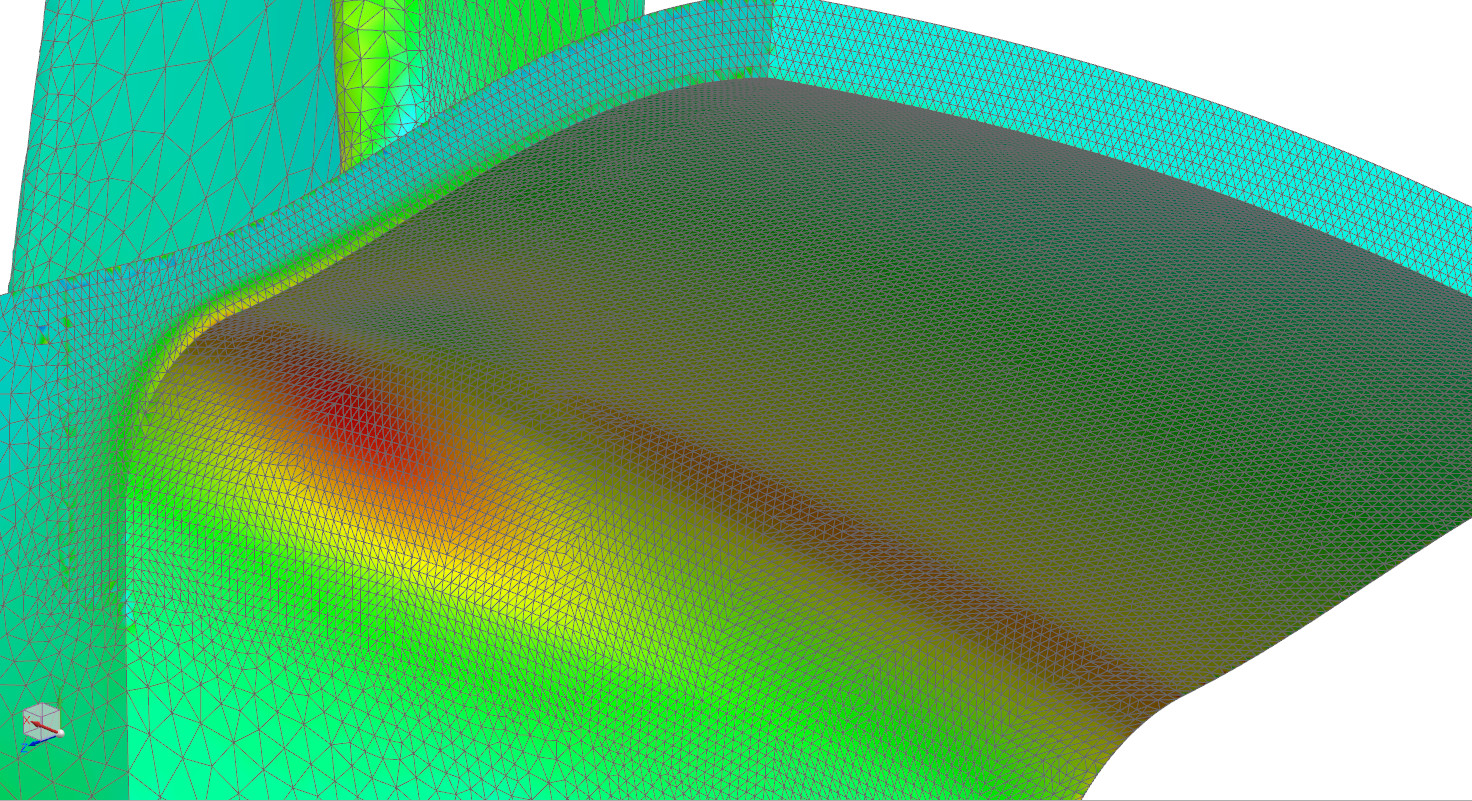
\includegraphics[width=0.8\linewidth]{Figures/0_075OriginalOperating.PNG}
 	\caption{Stator with stresses during operating conditions}
    \label{stator2}
 \end{figure}

The stator will crack at that point due to the resulting stress of the temperature differences between the lower part and the middle part of the stator. In this situation, the difference is about 400 [\textdegree C], which is the highest temperature difference in the stator. The lower temperature of the bottom part of the stator will cause it to expand more than the higher middle part of the stator; this will cause a tension between the bottom part and lower middle part of the stator. This tension is the highest around the edge between the bottom backside and the thin tail part of the stator because the thin tail part of the stator has much less material to distribute the tension to.

The highest stress found during the working condition is around 2217 [MPa] nodal and 2032 [MPa] elemental stress. This value is valid due to the fact that it has a convergence percentage of 8.3 \%, which is below the 10 \% convergence aimed for.
\newpage